\subsection{CR Alternativi: CyTrONE}\label{cr-alternativi-cytrone}

\textbf{CyTrONE}\footnote{\label{fn:ref_10}\url{https://github.com/crond-jaist/cytrone}}
e\textquotesingle{} un framework incentrato sul training che integra
contemporaneamente sia una piattaforma educativa che un Cyber Range.

La seguente immagine mostra i componenti di CyTrONE:

\begin{figure}[htbp]
  \centering
  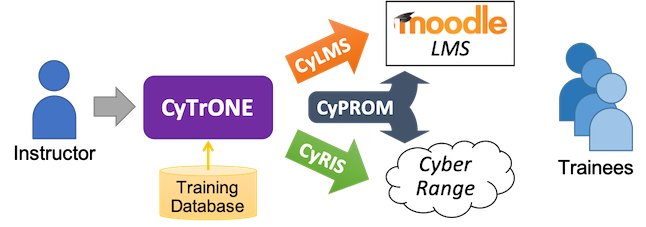
\includegraphics[width=0.85\linewidth,height=0.65\textheight,keepaspectratio]{src/images/cytrone-architecture.png}
  \caption{Cytrone Architecture}
  \label{fig:cytrone-architecture}
\end{figure}


\begin{itemize}
\tightlist
\item
  \textbf{CyLMS}: si occupa d icaricare il contenuto per il training su
  un Learning Management System come \textbf{Moodle}
\item
  \textbf{CyRIS} (Cyber Range Instantiation System): si occupa di
  istanziare l\textquotesingle ambiente di training su cui gli studenti
  possono condurre opportuni test per avanzare nel training.
\item
  \textbf{CyPROM}: si occupa di tracciare l\textquotesingle avanzamento
  controllando LMS ed il Cyber Range.
\end{itemize}

CyTrONE gestisce tre tipi di training\footnote{\label{fn:ref_11}\url{https://www.sciencedirect.com/science/article/pii/S0167404818306527}}:

\begin{itemize}
\tightlist
\item
  Training \emph{Attack-oriented}: si basa sul capire come riprodurre
  attacchi a vulnerabilita note.
\item
  Training \emph{Analysis-oriented}: si concentra
  sull\textquotesingle analisi dell\textquotesingle attacco, per capire
  come funziona e le sue conseguenze.
\item
  Training \textbf{Defense-oriented}: si conentra sulle tecniche di
  patching delle vulnerabilita, al fine di proteggere il sistema.
\end{itemize}

Quindi l\textquotesingle esperienza utente si concentra sul fatto che
gli studenti possono eseguire un training e visualizzare le risorse
associate sul Moodle ed al tempo stesso accedere al Cyber Range
associato.

CyTrONE si applica bene facendo le seguenti assunzioni:

\begin{quote}
\begin{enumerate}
\def\labelenumi{\arabic{enumi})}
\tightlist
\item
  \emph{L\textquotesingle obiettivo di ciascuna attività di formazione
  può essere formulato come un problema, che può dipendere o meno da
  altri problemi della stessa lezione (es: trova
  l\textquotesingle indirizzo IP, trova la flag);} \footref{fn:ref_11}
\end{enumerate}
\end{quote}

\begin{quote}
\begin{enumerate}
\def\labelenumi{\arabic{enumi})}
\setcounter{enumi}{1}
\tightlist
\item
  \emph{Il sistema è in grado di stabilire automaticamente se il
  partecipante abbia risolto il problema, confrontando la risposta
  fornita con un valore noto} \footref{fn:ref_11}
\end{enumerate}
\end{quote}

L\textquotesingle architettura di CyTrONE e\textquotesingle{} supportata
da un \emph{Training Database}, che si occupa di tenere in memoria le
informazioni per i vari training, che vengono caricate su CyTrONE da una
figura identificata come \emph{Training Coordinator}.Le informazioni
mantenute nel database sono per esempio: il training content, file e
programmi, macchine virtuali, ecc... \footref{fn:ref_11}

CyTrONE utilizza un file YAML per definire il contenuto di un training:

\begin{figure}[htbp]
  \centering
  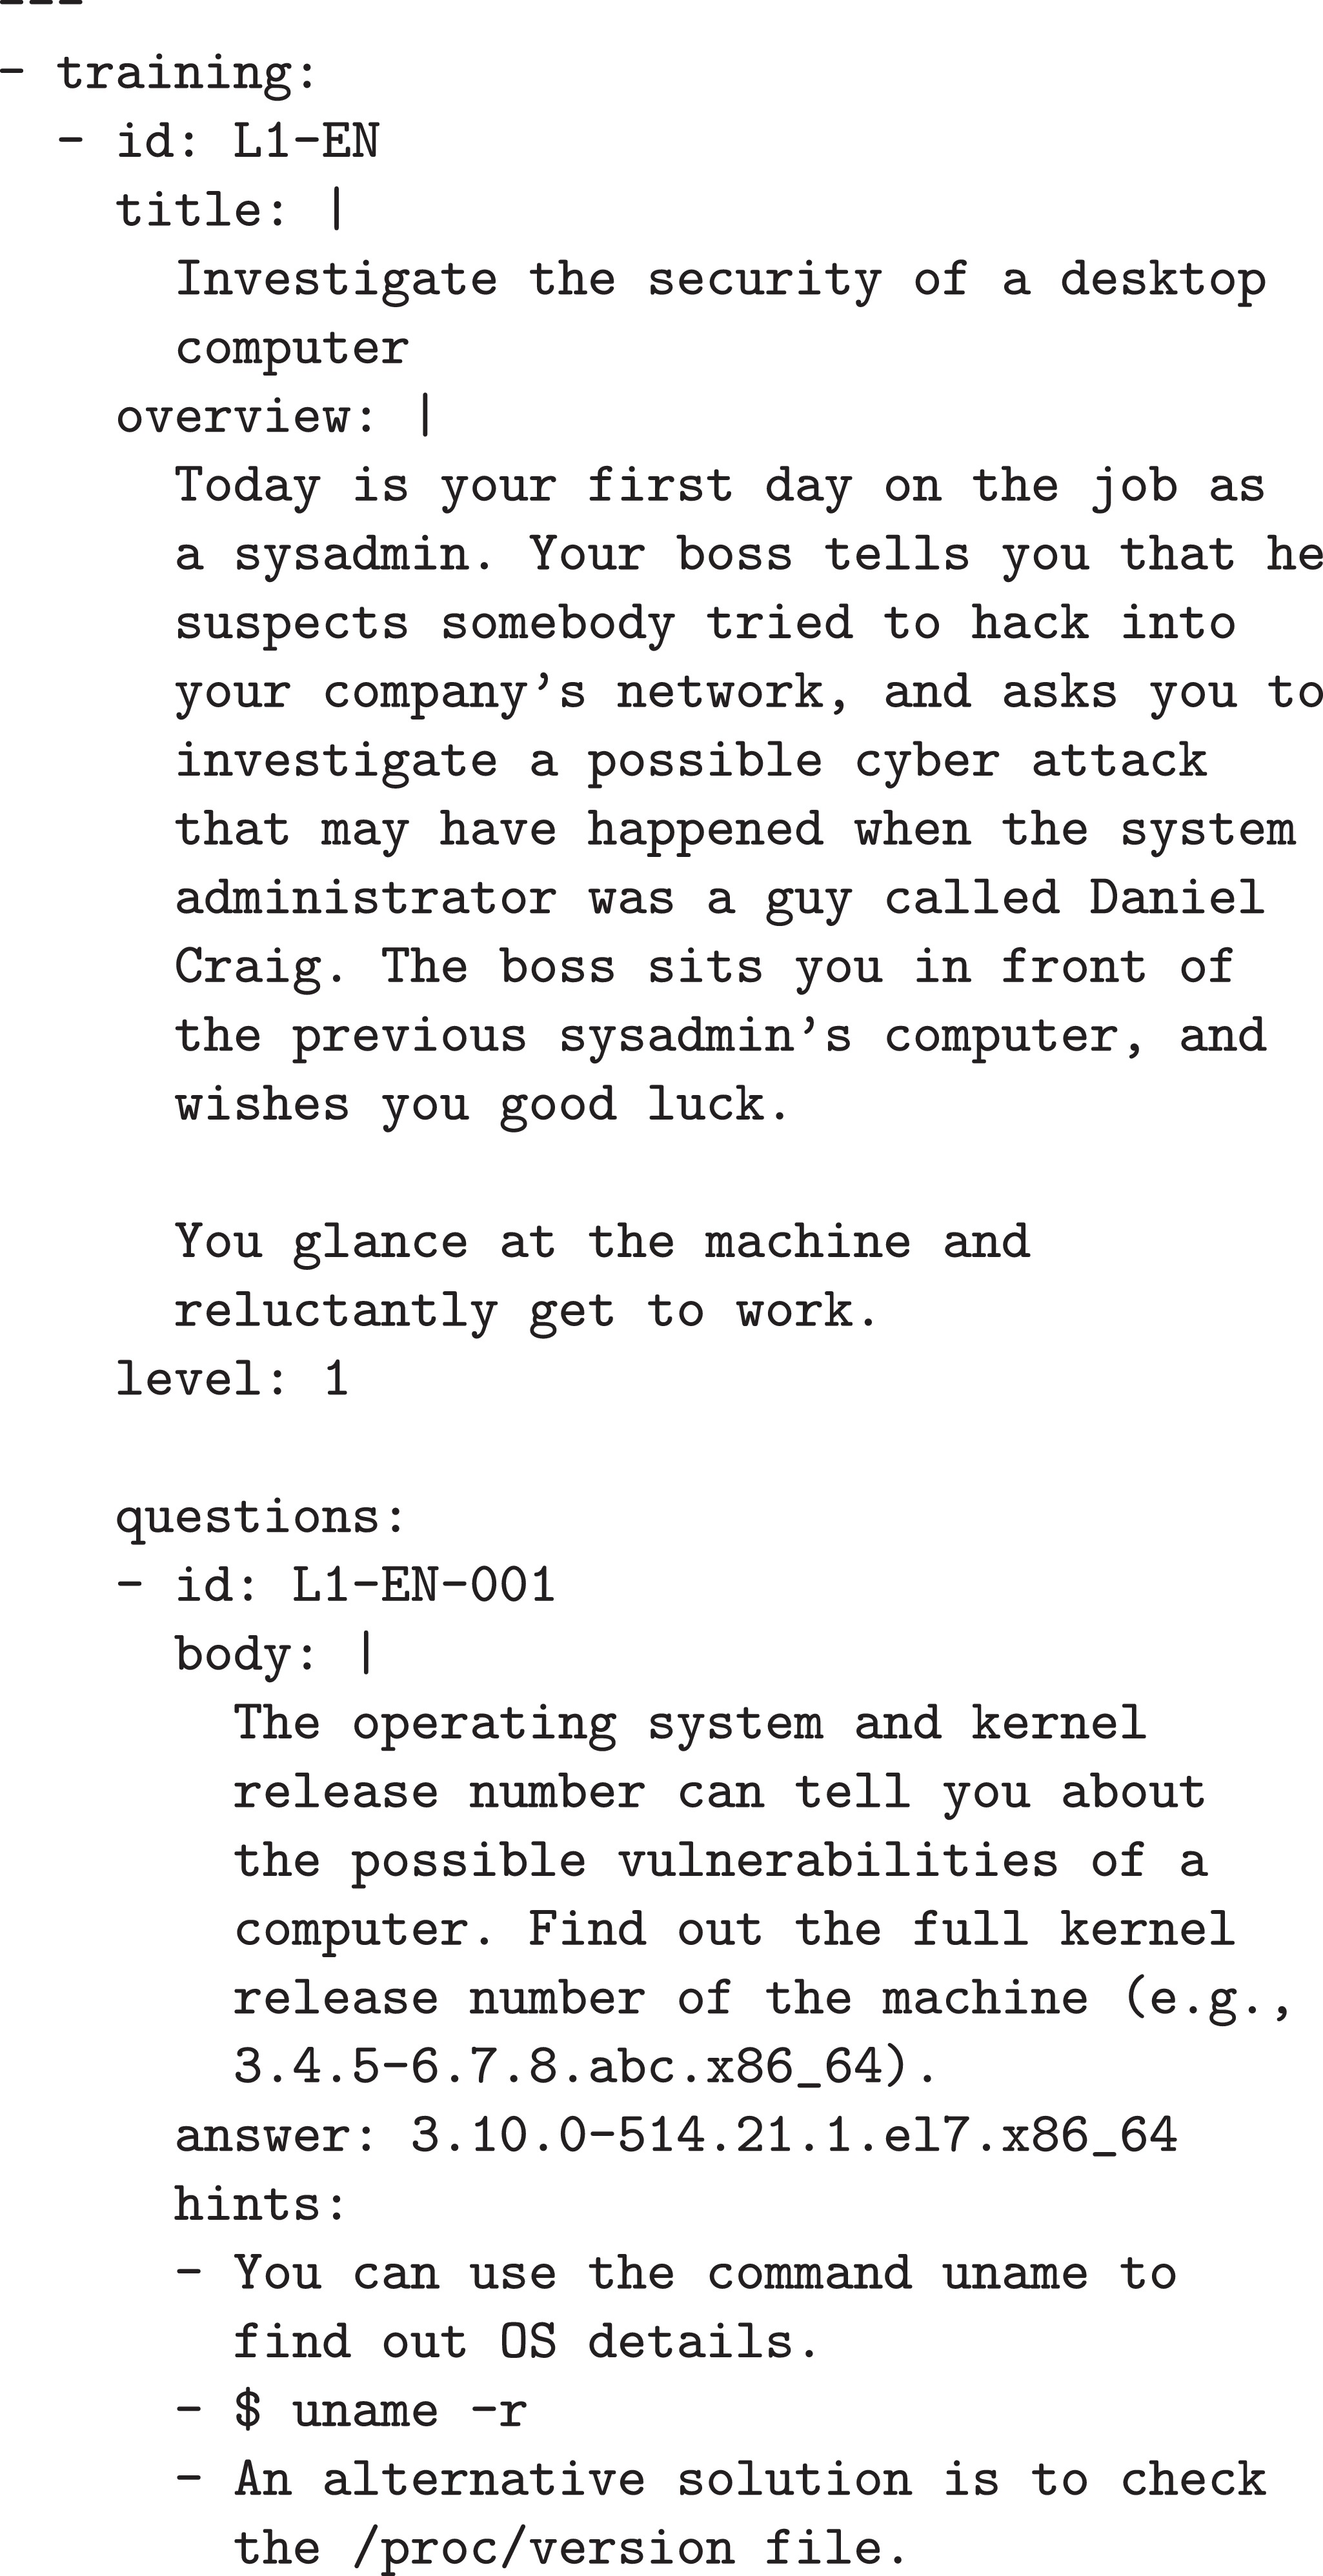
\includegraphics[width=0.85\linewidth,height=0.65\textheight,keepaspectratio]{src/images/cytrone-training.png}
  \caption{Cytrone Training}
  \label{fig:cytrone-training}
\end{figure}


E similmente, si usa un file YAML per definire la specifica del Cyber
Range: 
\begin{figure}[htbp]
  \centering
  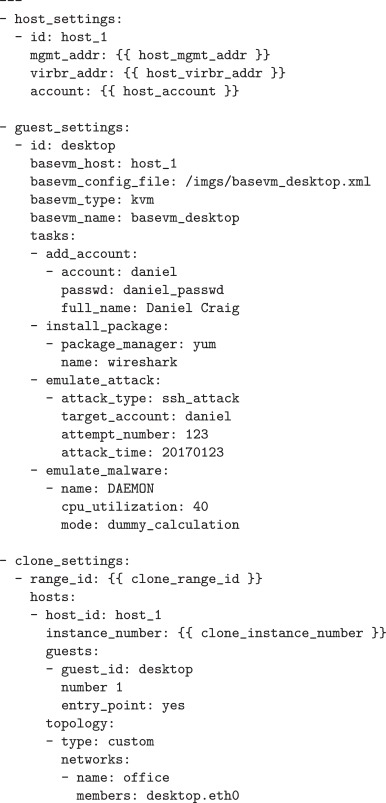
\includegraphics[width=0.85\linewidth,height=0.65\textheight,keepaspectratio]{src/images/cytrone-cyberrange.png}
  \caption{Cytrone Cyberrange}
  \label{fig:cytrone-cyberrange}
\end{figure}


A partire dalla configurazione YAML del Cyber Range, il sotto-sistema
CyRIS si occupa di istanziarlo. Successivamente, in caso di un training
\textbf{Defense-oriented} l\textquotesingle utente richiede
l\textquotesingle attacco associato alla vulnearbilita
all\textquotesingle interno del sistema e ne viene registrato
l\textquotesingle esisto.

Tutta via, sebbene il sistema sia ben ingegnerizzato soffre di alcuni
problemi:

\begin{enumerate}
\def\labelenumi{\arabic{enumi}.}
\tightlist
\item
  Il deploy delle vulnerabilita avviene su macchine virtuali, che
  possono costituire un alto overhead in termini di risorse, ed tempi di
  approvvigionamento lunghi per l\textquotesingle infrastruttura.
\item
  Il payload viene inviato remotamente dal
  \passthrough{\lstinline!cyberattack controller!} (che non fa altro che
  eseguire \passthrough{\lstinline!Metasploit!}). Tutta via il traffico
  di rete puo\textquotesingle{} essere intercettato dallo studente,
  ottenendo cosi suggerimenti per la soluzione.
\item
  L\textquotesingle esecuzione del payload puo scatenare la produzione
  di file log accessibili allo studente.
\item
  Necessita di un LMS (per design) per tenere traccia del training
  progress.
\end{enumerate}

TODO: analisi del grafico!
